% This template was minimally adapted from Steven V. Miller's template for academic manuscripts. See:
% http://svmiller.com/blog/2016/02/svm-r-markdown-manuscript/
\documentclass[]{article}
\usepackage[left=1in,top=1in,right=1in,bottom=1in]{geometry}
\newcommand*{\authorfont}{\fontfamily{phv}\selectfont}
\usepackage{lmodern}


\usepackage[T1]{fontenc}
\usepackage[utf8]{inputenc}

\newlength{\cslhangindent}
\setlength{\cslhangindent}{1.5em}
\newenvironment{CSLReferences}%
  {}%
  {\par}

\usepackage{abstract}
\renewcommand{\abstractname}{}    % clear the title
\renewcommand{\absnamepos}{empty} % originally center

\renewenvironment{abstract}
 {{%
    \setlength{\leftmargin}{0mm}
    \setlength{\rightmargin}{\leftmargin}%
  }%
  \relax}
 {\endlist}

\makeatletter
\def\@maketitle{%
  \newpage
%  \null
%  \vskip 2em%
%  \begin{center}%
  \let \footnote \thanks
    {\fontsize{18}{20}\selectfont\raggedright  \setlength{\parindent}{0pt} \@title \par}%
}
%\fi
\makeatother




\setcounter{secnumdepth}{0}

\usepackage{longtable,booktabs}

\usepackage{graphicx,grffile}
\makeatletter
\def\maxwidth{\ifdim\Gin@nat@width>\linewidth\linewidth\else\Gin@nat@width\fi}
\def\maxheight{\ifdim\Gin@nat@height>\textheight\textheight\else\Gin@nat@height\fi}
\makeatother
% Scale images if necessary, so that they will not overflow the page
% margins by default, and it is still possible to overwrite the defaults
% using explicit options in \includegraphics[width, height, ...]{}
\setkeys{Gin}{width=\maxwidth,height=\maxheight,keepaspectratio}


\title{Income as a Determinant of the Speed of Transmission: Study of
the Fifth Wave of SARS-CoV-2 in Toronto, Ontario  }
 



\author{\Large Jason
Lam\vspace{0.05in} \newline\normalsize\emph{400201299}   \and \Large Emily
Fletcher\vspace{0.05in} \newline\normalsize\emph{400210334}   \and \Large Syed
Hammad
Uddin\vspace{0.05in} \newline\normalsize\emph{400188361}   \and \Large Jenny
Chau\vspace{0.05in} \newline\normalsize\emph{400233137}   \and \Large Pierce
Bourgeois\vspace{0.05in} \newline\normalsize\emph{400220858}  }


\date{}

\usepackage{titlesec}

\titleformat*{\section}{\normalsize\bfseries}
\titleformat*{\subsection}{\normalsize\itshape}
\titleformat*{\subsubsection}{\normalsize\itshape}
\titleformat*{\paragraph}{\normalsize\itshape}
\titleformat*{\subparagraph}{\normalsize\itshape}





\newtheorem{hypothesis}{Hypothesis}
\usepackage{setspace}


% set default figure placement to htbp
\makeatletter
\def\fps@figure{htbp}
\makeatother


% move the hyperref stuff down here, after header-includes, to allow for - \usepackage{hyperref}

\makeatletter
\@ifpackageloaded{hyperref}{}{%
\ifxetex
  \PassOptionsToPackage{hyphens}{url}\usepackage[setpagesize=false, % page size defined by xetex
              unicode=false, % unicode breaks when used with xetex
              xetex]{hyperref}
\else
  \PassOptionsToPackage{hyphens}{url}\usepackage[draft,unicode=true]{hyperref}
\fi
}

\@ifpackageloaded{color}{
    \PassOptionsToPackage{usenames,dvipsnames}{color}
}{%
    \usepackage[usenames,dvipsnames]{color}
}
\makeatother
\hypersetup{breaklinks=true,
            bookmarks=true,
            pdfauthor={Jason Lam (400201299) and Emily
Fletcher (400210334) and Syed Hammad Uddin (400188361) and Jenny
Chau (400233137) and Pierce Bourgeois (400220858)},
             pdfkeywords = {Income, Toronto, COVID-19, Spatial
Statisitics, Spatial Analysis},  
            pdftitle={Income as a Determinant of the Speed of
Transmission: Study of the Fifth Wave of SARS-CoV-2 in Toronto,
Ontario},
            colorlinks=true,
            citecolor=blue,
            urlcolor=blue,
            linkcolor=magenta,
            pdfborder={0 0 0}}
\urlstyle{same}  % don't use monospace font for urls

% Add an option for endnotes. -----


% add tightlist ----------
\providecommand{\tightlist}{%
\setlength{\itemsep}{0pt}\setlength{\parskip}{0pt}}

% add some other packages ----------

% \usepackage{multicol}
% This should regulate where figures float
% See: https://tex.stackexchange.com/questions/2275/keeping-tables-figures-close-to-where-they-are-mentioned
\usepackage[section]{placeins}


\begin{document}
	
% \pagenumbering{arabic}% resets `page` counter to 1 
%    

% \maketitle

{% \usefont{T1}{pnc}{m}{n}
\setlength{\parindent}{0pt}
\thispagestyle{plain}
{\fontsize{18}{20}\selectfont\raggedright 
\maketitle  % title \par  

}

{
   \vskip 13.5pt\relax \normalsize\fontsize{11}{12} 
\textbf{\authorfont Jason
Lam} \hskip 15pt \emph{\small 400201299}   \par \textbf{\authorfont Emily
Fletcher} \hskip 15pt \emph{\small 400210334}   \par \textbf{\authorfont Syed
Hammad
Uddin} \hskip 15pt \emph{\small 400188361}   \par \textbf{\authorfont Jenny
Chau} \hskip 15pt \emph{\small 400233137}   \par \textbf{\authorfont Pierce
Bourgeois} \hskip 15pt \emph{\small 400220858}   

}

}






\vskip -8.5pt


 % removetitleabstract

\noindent  

\hypertarget{introduction}{%
\section{Introduction}\label{introduction}}

Since the first cases in 2019, the COVID-19 outbreak has taken the world
by storm. As of writing this (April 2022), there are over five hundred
million cases reported worldwide (World Health Organization 2022). With
its ability to rapidly spread, the COVID-19 has had profound
consequences in every facet of public and private life. Among these
include medical, economic, and social spaces (Baena-Díez et al. 2020).
Most importantly, these unsettling times have shone a light on
pre-existing disparities within national health systems. For many
researchers, this does not come as a surprise as socioeconomic factors
influencing health outcomes have been noted ubiquitously throughout the
world (Khalatbari-Soltani et al. 2020). According to Khalatbari-Soltani
et al.~(2020), there is even a link between those socio-economically
disadvantaged and increased risk of infectious disease.\\
This research continues in a vein of spatial statistical studies which
analyze COVID-19 incidence rates paired with a socio-economic factor.
Building upon Khalatabari-Soltani, et al.~(2020) and the socio-economic
position (SEP) framework, this study seeks to examine the relationship
between income levels, population density, and proportion of young
adults against COVID-19 incidence rates. More specifically, the
overarching objective of this study is to analyze the relationship
between the noted socio-economic variables and incidence rates of
COVID-19 during the fifth wave in Toronto, Ontario, Canada.

\hypertarget{background}{%
\section{Background}\label{background}}

\hypertarget{factors-related-to-covid-19-incidence}{%
\subsection{Factors Related to COVID-19
Incidence}\label{factors-related-to-covid-19-incidence}}

A person's income level affects how they go about their everyday lives.
The associated behavioural pattern has been linked to change in health
outcomes (Khalatbari-Soltani et al. 2020). Low income, for example,
affects housing condition and leads to more tight housing arrangements.
Such factors have been associated in the increased risk of infections
for pathogens such as tuberculosis (Khalatbari-Soltani et al. 2020).

In Ontario, from January 21 to June 30, 2022, the most attributed
workplace was manufacturing (Murti et al. 2021). Manufacturing accounted
for 45\% of outbreaks which totaled 65\% of outbreak cases. Another
notable sector was Transport and Warehousing (11\% of outbreaks, 8\% of
outbreak cases). In Toronto, it has been observed the COVID-19 first
infiltrate in high income communities before quickly spreading to lower
income communities (Mishra et al. 2022). According to Mishra et
al.~(2022) lower income neighbourhoods were also defined by their higher
dwelling densities and greater proportion of occupations that could not
make the transition to remote work.

In addition, the susceptibility of adolescents (aged 10-19 years) and
youth (aged 15-24 years) to COVID-19 has been a controversial research
topic since the pandemic began (Rumain, Schneiderman, and Geliebter
2021). While several studies have concluded that young adults are
significantly less susceptible to COVID-19 than older adults, others
have found that the prevalence of COVID-19 for adolescents and youth to
be significantly greater than that of older adults (Rumain,
Schneiderman, and Geliebter 2021). In April 2021, COVID-19 cases were
rising rapidly for young Canadians, with cases being highest among those
aged 20 to 39 (Aziz 2021). Suggested factors that attribute to higher
COVID-19 incidence among younger people include the reopening of high
schools, colleges, and universities, larger and more frequent social
gatherings and non-compliance with public health guidelines due to
perceived low-risk of severe symptoms for the age group, and low income.
(Aleta and Moreno 2020). Health-related behaviours of younger adults may
also affect their susceptibility to COVID-19 infection (Abbasi 2020). In
an online national survey of adolescents and young adults, vaping and
the dual use of e-cigarettes and cigarettes heavily increased the
chances of COVID-19 diagnosis (Gaiha, Cheng, and Halpern-Felsher 2020).

Lastly, Toronto has the densest urban core in the province and is one of
the most densely populated regions in North America. This has made it
susceptible to the ability of COVID-19 to rapidly spread. To date, there
have been more than 300,000 reported cases with more than 4000 deaths
(City of Toronto 2021). Within the city, there are several pockets that
are denser than others, and this density is an important factor to look
at. Population density is a measure of spatial distribution of people
across space. In the case of Toronto, St James Town is the most densely
populated neighbourhood in the city (Canadian Urban Institute 2016).
Research around population density and its link to COVID-19
susceptibility is limited. Past literature has not shown a clear
relationship between the two, with some noting a positive correlation
(Hamidi and Hamidi 2021) while others deducing an insignificant
relationship {[}Carozzi\_Provenzano\_Roth\_2020{]}. This, as suggested
by the entire catalogue of research, is connected to the regional
variations connected to density. Some denser areas may have better
services to limit their exposure to the virus, while others may be
poorer and so may be more susceptible to the virus. It is important to
explore this phenomenon in the context of Toronto, to understand the
type of relationship found in the city.

\hypertarget{covid-19-waves-in-toronto}{%
\subsection{COVID-19 Waves in Toronto}\label{covid-19-waves-in-toronto}}

The first case of COVID-19 in Ontario (and Canada) was reported on
January 25, 2020 (Nielsen 2020). As the virus began to spread, Ontario
entered its first wave of COVID-19 on February 26, 2020. The first wave
of COVID-19 lasted 188 days, ending on August 31, 2020 (Public Health
Ontario 2021). As Ontario began loosening restrictions as part of its
3-stage reopening plan, people started getting together again, and
observed cases began to rise. Ontario's second wave began September 2020
and ended in February 2021, with cases peaking in January 2021 (Public
Health Ontario 2021). The third wave in Ontario was driven by the Alpha
(B.1.1.7) variant, which was more transmissible (Detsky and Bogoch
2021). The third wave lasted from March to July 2021, and was the
largest wave yet, with the peak number of new cases in a day in Ontario
being 5067 (Public Health Ontario 2022). The emergence of the Delta
variant (B.1.617.2) caused a smaller and shorter fourth wave in Ontario
that lasted from August to October 2021. The largest number of new cases
reported in a day in Ontario during the fourth wave was 878.

\begin{longtable}[]{@{}
  >{\raggedright\arraybackslash}p{(\columnwidth - 10\tabcolsep) * \real{0.06}}
  >{\raggedright\arraybackslash}p{(\columnwidth - 10\tabcolsep) * \real{0.23}}
  >{\raggedright\arraybackslash}p{(\columnwidth - 10\tabcolsep) * \real{0.18}}
  >{\raggedright\arraybackslash}p{(\columnwidth - 10\tabcolsep) * \real{0.17}}
  >{\raggedright\arraybackslash}p{(\columnwidth - 10\tabcolsep) * \real{0.23}}
  >{\raggedright\arraybackslash}p{(\columnwidth - 10\tabcolsep) * \real{0.14}}@{}}
\caption{Waves of COVID-19 in Ontario}\tabularnewline
\toprule
\begin{minipage}[b]{\linewidth}\raggedright
Wave
\end{minipage} & \begin{minipage}[b]{\linewidth}\raggedright
Associated Variant
\end{minipage} & \begin{minipage}[b]{\linewidth}\raggedright
Approx. Start
\end{minipage} & \begin{minipage}[b]{\linewidth}\raggedright
Approx. End
\end{minipage} & \begin{minipage}[b]{\linewidth}\raggedright
Peak Cases Per Day
\end{minipage} & \begin{minipage}[b]{\linewidth}\raggedright
Total Cases
\end{minipage} \\
\midrule
\endfirsthead
\toprule
\begin{minipage}[b]{\linewidth}\raggedright
Wave
\end{minipage} & \begin{minipage}[b]{\linewidth}\raggedright
Associated Variant
\end{minipage} & \begin{minipage}[b]{\linewidth}\raggedright
Approx. Start
\end{minipage} & \begin{minipage}[b]{\linewidth}\raggedright
Approx. End
\end{minipage} & \begin{minipage}[b]{\linewidth}\raggedright
Peak Cases Per Day
\end{minipage} & \begin{minipage}[b]{\linewidth}\raggedright
Total Cases
\end{minipage} \\
\midrule
\endhead
1st & Original Strain & February 2020 & August 2020 & 752 & 42,486 \\
2nd & Original Strain & September 2020 & February 2021 & 4,168 &
260,643 \\
3rd & Alpha & March 2021 & July 2021 & 5,067 & 24,7654 \\
4th & Delta & August 2021 & October 2021 & 878 & 49,704 \\
5th & Omicron & December 2022 & February 2022 & 19,373 & 469,955 \\
\bottomrule
\end{longtable}

The fifth wave of the pandemic lasted from the beginning of December
2021 until mid-February 2022. The catalyst for this was the emergence of
a new, highly transmissible variant called Omicron. The variant, which
was first reported globally in November 2021, has been thoroughly
researched due to its scale and rate of infection. This research
suggests that the variant is highly transmissible due to several
factors. This includes the fact that Omicron is more likely to evade
immunity from a previous infection, meaning that there is a high chance
that you can get re-infected with COVID-19 (Pulliam et al. 2021). Other
research suggests that the variant is up to 3.7\% more infectious among
vaccinated citizens than its predecessors (Mohsin and Mahmud 2022).
During the fifth wave, it became the dominant strain and was responsible
for 95\% infections globally. In Ontario, the first Omicron cases were
reported on November 28, 2021 (Government of Ontario 2021). During the
Omicron wave, the highest number of new cases reported for a single day
in the province was 19,373 (Public Health Ontario 2022).

This study will determine how average income, proportion of youths, and
population density may affect the change in COVID-19 case rates between
the first and last week of December 2021.

\hypertarget{study-area}{%
\section{Study area}\label{study-area}}

The analysis was conducted at the neighbourhood level for the City of
Toronto (See Figure 1). `Neighbourhood' is a geographic level
specifically designed by the City of Toronto. They were created by city
to help government and other planning organizations with obtaining
socio-economic data (City of Toronto 2017). In total there are 140
unique areas, and their boundaries are based on the Canadian Census
Track. Each neighbourhood may contain between two to five of these
census tracts. The geography of neighbourhood was chosen for this study,
as opposed to wards or dissemination blocks, not only to showcase acute
changes within populations but due to the availability of both COVID-19
and the socio-economic data. The large number neighbourhoods also enable
this study to capture diversity across the city.

\begin{figure}
\centering
\includegraphics{Final-Project_files/figure-latex/unnamed-chunk-4-1.pdf}
\caption{Neighbourhoods in Toronto, Ontario, Canada}
\end{figure}

\hypertarget{data}{%
\section{Data}\label{data}}

The shapefile used to delineate and map Toronto's neighbourhoods in this
study was obtained from the ``Neighbourhoods'' file in the City of
Toronto Open Data portal (City of Toronto 2022). Using the same portal,
the COVID-19 data was retrieved from the dataset ``COVID-19 Cases in
Toronto'' (Toronto Public Health 2022). The data was downloaded as a
comma-separated values (CSV) file. This data is updated weekly by the
city and reports each individual case as a record. The time period of
interest was December 2021, corresponding to a peak in COVID-19 cases
within the fifth wave of the pandemic in Ontario. The cases from the
first week of December 2021 (Dec.~1 - Dec.~7) and the last week (Dec.~25
- Dec.~31) were filtered out and aggregated by neighbourhood. The
average income, percentage of youth (18-24), and population density of
each neighbourhood that was used in this study was derived from data in
the ``Neighbourhood Profile'' dataset retrieved from Toronto Open Data
(Toronto Social Development, Finance \& Administration 2011). This
dataset documents demographic and socioeconomic information for each of
Toronto's neighbourhoods, including total population and the number of
people of each age, using Canada's census data held every 5 years.

\hypertarget{methods}{%
\section{Methods}\label{methods}}

This study used RStudio to conduct the data pre-processing, that is
cleaning of the original datasets. A unique method was ran to covered
the date data in the COVID-19 case table into character data type. This
was so the records could be parsed in respect to this studies period of
interest.

The analysis was also done in RStudio using several R packages,
including spatstat, tidyverse, ggplot2, dplyr, gridExtra, patchwork, and
spdep to analyze the area data and find a potential relationship between
the chosen independent variables (average income, percentage of 18-24
year old individuals, population density) and the dependent variable
(fold change in COVID-19 case rates from the first to last week of
December 2021) for the neighbourhoods of Toronto. For the initial
visualization and analysis of the area data, choropleth maps and Moran's
I were used to identify patterns in the data. Then, to gain more insight
on the process behind these patterns, regression analysis was used to
determine the relationship between the independent and dependent
variables.

This document was also written and exported through R-Markdown with
minimal adaptation from Steven V. Miller's template for academic
manuscripts. See:
\url{http://svmiller.com/blog/2016/02/svm-r-markdown-manuscript/}{[}\url{https://github.com/svmiller/svm-r-markdown-templates/blob/master/svm-latex-ms.tex}{]}
and
(\url{https://github.com/svmiller/svm-r-markdown-templates/blob/master/svm-latex-ms.tex})

The data and code used in this project can be found on Github:
\url{https://github.com/lamj54/4GA3-Project}. This document is also
available as a RMarkdown file, which includes both the code and the text
used to create this report.

\hypertarget{analysis}{%
\section{Analysis}\label{analysis}}

\hypertarget{data-exploration}{%
\subsection{Data Exploration}\label{data-exploration}}

First, to obtain a preliminary understanding of trends in the data,
choropleth maps were used to visualize the fold change in COVID-19 cases
between the first and last week of December 2021 (Figure 2), per capita
income (Figure 3), population density (Figure 4), and the proportion of
18- to 24-year-old individuals in each neighbourhood in Toronto (Figure
5).

\begin{figure}
\centering
\includegraphics{Final-Project_files/figure-latex/unnamed-chunk-20-1.pdf}
\caption{The change in COVID-19 rates (cases per 10,000) between the
first and last week of December 2021 in Toronto by neighbourhood}
\end{figure}

In Figure 2, it can be seen that the fold change for all neighbourhoods
in Toronto is positive, indicating that they all experienced an increase
in COVID-19 case rates in the last week of December 2021 compared to the
first week of December 2021. In particular, the neighbourhoods coloured
in a darker red and orange showed a significantly large fold change in
COVID-19 rates in comparison to other neighbourhoods, which possibly
signifies the location of COVID-19 hotspots during December 2021.
Accordingly, the neighbourhoods located close to such spots seem to have
relatively large fold changes as well, as shown through their light
orange colour. Neighbourhoods with smaller fold changes, seen in yellow
in the map, appear to be located further away from areas with more
intense fold changes.

\begin{figure}
\centering
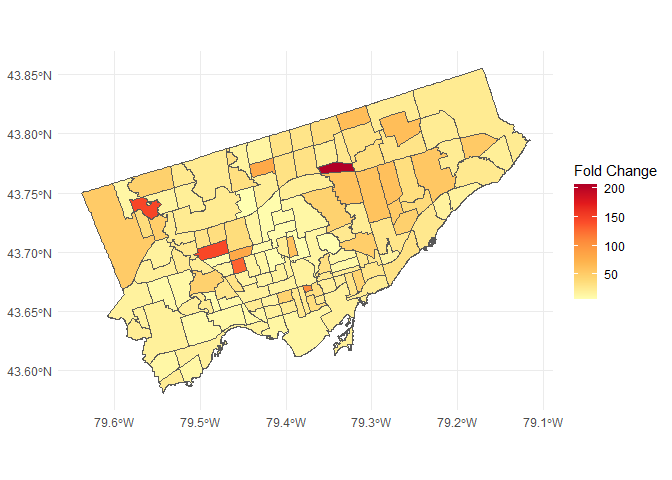
\includegraphics{Final-Project_files/figure-latex/unnamed-chunk-21-1.pdf}
\caption{The average income of individuals in Toronto by neighbourhood}
\end{figure}

Neighbourhoods with greater average income appear darker in colour on
the map in Figure 3, showing that people with higher income tend to
concentrate near the center of Toronto. Other neighbourhoods with high
average income can be seen in the west of Toronto as well.

From a visual comparison of Figures 2 and 3, it looks like the
neighbourhoods with higher average incomes have lower fold changes in
COVID-19 case rates while the neighbourhoods with high fold changes are
those with lower average incomes.

\begin{figure}
\centering
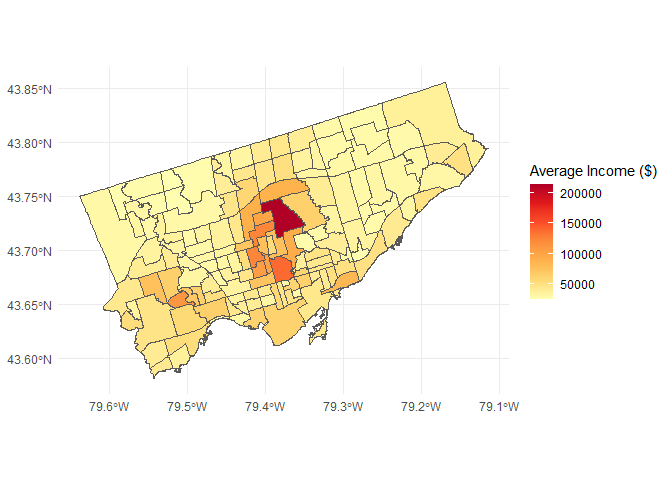
\includegraphics{Final-Project_files/figure-latex/unnamed-chunk-22-1.pdf}
\caption{The population density of each of Toronto's neighbourhoods}
\end{figure}

From Figure 4, it seems that there may be a greater population density
in some of the neighbourhoods located towards the southern areas of
Toronto. Population density appears to be lower in neighbourhoods
located in the outskirts of the city. Comparing Figures 2 and 4, the
neighbourhoods with very large fold changes do not have particularly
high population densities, and the neighbourhoods with high population
densities do not seem to have very high fold changes. Neighbourhoods
with similar population densities appear to have different changes in
COVID-19 case rates, which may indicate that its relationship with
population density is very weak.

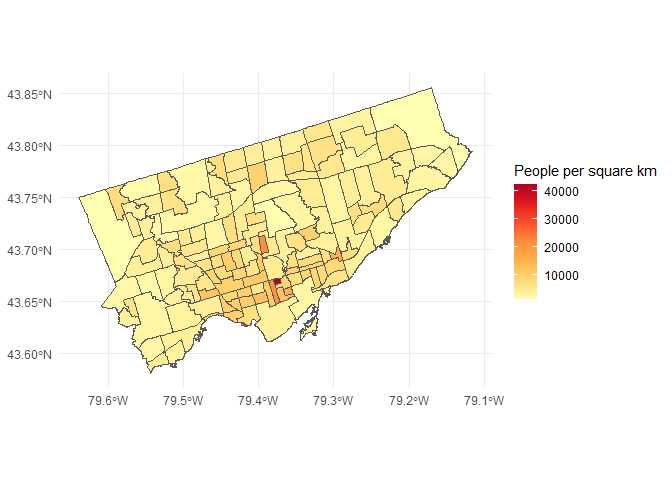
\includegraphics{Final-Project_files/figure-latex/unnamed-chunk-23-1.pdf}
Looking at Figure 5, there are a cluster of neighbourhoods in the south
of Toronto, coloured in red, that have a particularly high percentage of
18- to 24-year-old individuals making up their population. In addition,
a neighbourhood located near the north, in dark orange, has a relatively
high proportion of 18- to 24-year-old individuals. Comparing this map to
Figure 2, it seems that the neighbourhoods with higher percentages of
youth have lower changes in COVID-19 case rates. Accordingly, the
neighbourhoods with high fold changes have a relatively small percentage
of youth in them. These observations may suggest that the percentage of
youth in a neighbourhood is actually negatively correlated with change
in COVID-19 rates.

\hypertarget{spatial-autocorrelation}{%
\subsection{Spatial autocorrelation}\label{spatial-autocorrelation}}

Before doing a regression analysis to determine the relationship between
the change in COVID-19 case rates and the predictor variables, an
analysis of the pattern in the change in COVID-19 case rates must first
be done. If its pattern is non-random, then regression analysis can be
used to provide more information about the process that is creating this
pattern.

To test whether a spatial pattern is random or non-random, Moran's I, a
coefficient of spatial autocorrelation, can be calculated and used in a
hypothesis test that assesses for spatial randomness. The null
hypothesis of this test is that the pattern is spatially random.

The Moran's I statistic for this data is 0.089308782 and the p-value of
the test is 0.01787. Since the p-value is less than 0.05, it is
sufficiently small enough to reject the null hypothesis with a high
degree of confidence. This means that the change in COVID-19 case rates
is spatially autocorrelated, not spatially random. As well, since the
Moran's I statistic is positive, it suggests that it is a non-random
spatial pattern where high values tend to be with other high values, and
low values tend to be with other low values. This agrees with the visual
observation of the choropleth map of the change in COVID-19 case rates
in Figure 2.

\begin{figure}
\centering
\includegraphics{Final-Project_files/figure-latex/unnamed-chunk-27-1.pdf}
\caption{The categorization of neighbourhoods based on local Moran's I,
a statistic that describes the autocorrelation of a specific location
and its contribution to the global Moran's I statistic.}
\end{figure}

Correspondingly, the map of local Moran's I, which breaks down Moran's I
to examine the contribution of each area to the statistic, in Figure 6,
shows that neighbourhoods with high fold changes are surrounded by other
neighbourhoods that have high fold changes as well. Such regions are
labelled ``HH'' for ``High-High.'' On the other hand, the neighbourhoods
with low fold changes in COVID-19 case rates are surrounded by those
with similarly low fold changes, which are labelled ``LL'' for
``Low-Low.'' Other possible combinations are ``HL'' and ``LH''
(``High-Low'' and ``Low-High''). Categorizing each neighbourhood in this
way, in addition to showing whether a neighbourhood's local Moran's I is
statistically significant and thus spatially autocorrelated, reveals the
hot spots and cold spots that contribute significantly to the global
Moran's I statistic. From Figure 6, it can be seen that there are
several hot spots where COVID-19 case rates have increased
significantly, displayed in bright red on the map.

\hypertarget{regression-analysis}{%
\subsection{Regression Analysis}\label{regression-analysis}}

\hypertarget{results-of-the-model}{%
\subsubsection{Results of the Model}\label{results-of-the-model}}

Now knowing that the change in COVID-19 case rates in Toronto's
neighbourhoods is not spatially random, the question is what is the
process behind the creation of this pattern? To gain more insight on
this, a regression analysis can be used to determine the relationship
between several independent variables and the changes in COVID-19 case
rate.

\begin{table}[!htbp] \centering 
  \caption{Linear regression model of fold change in COVID-19 case rates with respect to income, percentage of 18- to 24-year-old individuals, and population density} 
  \label{} 
\begin{tabular}{@{\extracolsep{5pt}}lc} 
\\[-1.8ex]\hline 
\hline \\[-1.8ex] 
 & \multicolumn{1}{c}{\textit{Dependent variable:}} \\ 
\cline{2-2} 
\\[-1.8ex] & fold\_increase \\ 
\hline \\[-1.8ex] 
 Intercept, Average Income, Percentage of 18-24 year olds, Population Density & $-$0.0003$^{***}$ \\ 
  & (0.0001) \\ 
  & \\ 
 perc\_18\_24 & 0.980 \\ 
  & (1.122) \\ 
  & \\ 
 pop\_density & 0.001 \\ 
  & (0.001) \\ 
  & \\ 
 Constant & 29.225$^{**}$ \\ 
  & (12.026) \\ 
  & \\ 
\hline \\[-1.8ex] 
Observations & 140 \\ 
R$^{2}$ & 0.083 \\ 
Adjusted R$^{2}$ & 0.063 \\ 
Residual Std. Error & 26.759 (df = 136) \\ 
F Statistic & 4.112$^{***}$ (df = 3; 136) \\ 
\hline 
\hline \\[-1.8ex] 
\textit{Note:}  & \multicolumn{1}{r}{$^{*}$p$<$0.1; $^{**}$p$<$0.05; $^{***}$p$<$0.01} \\ 
\end{tabular} 
\end{table}

As seen in the results of the regression model in Table 2, the only
independent variable that is statistically significant in the model is
the average income of a neighbourhood. This is because the p-values for
average income, percentage of individuals aged 18-24, and population in
this model are 0.00462, 0.38397, and 0.28312 respectively. They indicate
whether or not the null hypothesis, which states that a variable is not
statistically significant in the regression model, should be rejected or
not. Since the p-value for average income is less than 0.05, it is small
enough to reject the null hypothesis with a high degree of confidence.
This means that average income helps to explain the variance in the
dependent variable, the change in COVID-19 case rates. On the other
hand, the p-values for percentage of 18- to 24-year-old individuals and
population density are large, leading to the null hypothesis being
accepted. As a result, these two variables do not contribute
significantly to the model. This result suggests that average income is
a factor that influences the pattern of changes in COVID-19 case rates
across Toronto's neighbourhoods, while the percentage of 18- to
24-years-old individuals and population density are not.

Moreover, Table 2 shows that the coefficient for average income is
approximately -0.0003 (0.0002591 exactly), indicating that
neighbourhoods with higher average incomes have smaller changes in
COVID-19 case rates. Thus, higher income causes the growth in COVID-19
cases to slow, while lower income causes the growth in COVID-19 cases to
accelerate. This agrees with our initial hypothesis. Individuals with
lower income tend to have less means to protect themselves from
COVID-19, due to factors such as lower income jobs being less
accommodating of remote work.

\hypertarget{model-diagnostics}{%
\subsubsection{Model Diagnostics}\label{model-diagnostics}}

To determine whether the model has successfully retrieved all of the
systematic pattern, its residuals need to be analyzed for randomness. If
the residuals are non-random, this means that the model has failed to
capture the entire pattern and must be adjusted to have random
residuals.

The residuals can first be visualized with a map by plotting the sign of
the residual for each neighbourhood (Figure 7). A positive residual
indicates that the model overestimates the change in COVID-19 case
rates, while a negative residual means that the model underestimates it.

\begin{figure}
\centering
\includegraphics{Final-Project_files/figure-latex/unnamed-chunk-29-1.pdf}
\caption{Map of the sign of the residuals from the regression model for
each neighbourhood}
\end{figure}

From a visual observation of Figure 7, there does not appear to be any
obvious clusters of positive or negative residuals. To obtain a more
concrete conclusion, the Moran's I coefficient can be used in a
hypothesis test again to test for spatial randomness.

The result of the Moran's I hypothesis test supports the visual
observation of Figure 7. The null hypothesis of the test is that the
pattern analyzed is spatially random. The p-value is 0.1871, which is
greater than 0.05 and thus large enough to accept the null hypothesis.
Consequently, the residuals of this regression model is random,
indicating that the model successfully capture all of the pattern within
the changes in COVID-19 case rates across Toronto's neighbourhoods. This
means that the model does not need to be adjusted since its assumption
that the residuals are independent has not been violated, so the results
obtained from the model (summarized in Table 2) are valid.

\hypertarget{conclusion}{%
\section{Conclusion}\label{conclusion}}

Overall, the changes in COVID-19 case rates across neighbourhoods in
Toronto show spatial autocorrelation, as found using Moran's I. A
regression analysis of the change in COVID-19 case rates with respect to
average income, percentage of 18- to 24-year-old individuals, and
population density was also done. It revealed that there is a connection
between average income and changes in the rates of COVID-19 cases, with
neighbourhoods with lower income having greater changes in COVID-19 case
rates. This means that a lower average income can quicken the growth in
COVID-19 cases. In addition, the results of the regression show that
other socio-economic factors, the percentage of 18- to 24-year olds and
the population density in a neighbourhood, did not have a clear
connection with the COVID-19 case changes. It is recommended that, for
the future, more research should be done on the relationship with
socio-economic variables and changes in COVID-19 cases. Socio-economic
factors are complex factors that need to be further explored to verify
the relationships found in this study.

Identifying groups of individuals from a socio-economic perspective is
the first step to establishing that a person's socioeconomic position
may be as much of an indicator in predicting health outcomes as a
pre-existing medical condition. In establishing such similarities,
governing healthcare bodies may extend precautionary recommendations to
people with specific socio-economic conditions, thus providing a more
in-depth and informed disease prevention plan. In a pursuit of
identifying groups of the populations who are more susceptible to poorer
outcomes when combating health problems, more research in this area
needs to be undertaken.

\hypertarget{references}{%
\section*{References}\label{references}}
\addcontentsline{toc}{section}{References}

\hypertarget{refs}{}
\begin{CSLReferences}{1}{0}
\leavevmode\vadjust pre{\hypertarget{ref-Abbasi_2020}{}}%
Abbasi, Jennifer. 2020. {``Younger Adults Caught in COVID-19 Crosshairs
as Demographics Shift.''} \emph{JAMA} 324 (21): 2141--43.
\url{https://doi.org/10.1001/jama.2020.21913}.

\leavevmode\vadjust pre{\hypertarget{ref-Aleta_Moreno_2020}{}}%
Aleta, Alberto, and Yamir Moreno. 2020. {``Age Differential Analysis of
COVID-19 Second Wave in Europe Reveals Highest Incidence Among Young
Adults,''} November, 2020.11.11.20230177.
\url{https://doi.org/10.1101/2020.11.11.20230177}.

\leavevmode\vadjust pre{\hypertarget{ref-Aziz_2021}{}}%
Aziz, Saba. 2021. {``{`Hit the Hardest'}: Why COVID-19 Cases Are Rising
Among Young Canadians - National \textbar{} Globalnews.ca.''}
\emph{Global News}.
\url{https://globalnews.ca/news/7731485/covid-variant-cases-young-canadians/}.

\leavevmode\vadjust pre{\hypertarget{ref-Baena-Diez_Barroso_Cordeiro-Coelho_Diaz_Grau_2020}{}}%
Baena-Díez, Jose Miguel, María Barroso, Sara Isabel Cordeiro-Coelho,
Jorge L. Díaz, and María Grau. 2020. {``Impact of COVID-19 Outbreak by
Income: Hitting Hardest the Most Deprived.''} \emph{Journal of Public
Health (Oxford, England)} 42 (4): 698--703.
\url{https://doi.org/10.1093/pubmed/fdaa136}.

\leavevmode\vadjust pre{\hypertarget{ref-CUI_2016}{}}%
Canadian Urban Institute. 2016. {``TOcore Neighbourhood Population
Profiles,''} July, 46.

\leavevmode\vadjust pre{\hypertarget{ref-Toronto_2017}{}}%
City of Toronto. 2017. {``Neighbourhood Profiles.''} \emph{City of
Toronto}. City of Toronto.
\url{https://www.toronto.ca/city-government/data-research-maps/neighbourhoods-communities/neighbourhood-profiles/}.

\leavevmode\vadjust pre{\hypertarget{ref-Toronto_2021}{}}%
---------. 2021. {``COVID-19: Case Counts.''} \emph{City of Toronto}.
City of Toronto.
\url{https://www.toronto.ca/home/covid-19/covid-19-pandemic-data/covid-19-weekday-status-of-cases-data/}.

\leavevmode\vadjust pre{\hypertarget{ref-Toronto_2022}{}}%
---------. 2022. {``Neighborhood Shapefile.''} Social Development,
Finance \& Administration.

\leavevmode\vadjust pre{\hypertarget{ref-Detsky_Bogoch_2021}{}}%
Detsky, Allan S., and Isaac I. Bogoch. 2021. {``COVID-19 in Canada:
Experience and Response to Waves 2 and 3.''} \emph{JAMA} 326 (12):
1145--46. \url{https://doi.org/10.1001/jama.2021.14797}.

\leavevmode\vadjust pre{\hypertarget{ref-Gaiha_Cheng_Halpern-Felsher_2020}{}}%
Gaiha, Shivani Mathur, Jing Cheng, and Bonnie Halpern-Felsher. 2020.
{``Association Between Youth Smoking, Electronic Cigarette Use, and
COVID-19.''} \emph{Journal of Adolescent Health} 67 (4): 519--23.
\url{https://doi.org/10.1016/j.jadohealth.2020.07.002}.

\leavevmode\vadjust pre{\hypertarget{ref-GofO_2021}{}}%
Government of Ontario. 2021. {``Ontario Confirms First Two Cases of
Omicron Variant.''} Government. \emph{News.ontario.ca}.
\url{https://news.ontario.ca/en/statement/1001241/ontario-confirms-first-two-cases-of-omicron-variant}.

\leavevmode\vadjust pre{\hypertarget{ref-Hamidi_Hamidi_2021}{}}%
Hamidi, Shima, and Iman Hamidi. 2021. {``Subway Ridership, Crowding, or
Population Density: Determinants of COVID-19 Infection Rates in New York
City.''} \emph{American Journal of Preventive Medicine} 60 (5): 614--20.
\url{https://doi.org/10.1016/j.amepre.2020.11.016}.

\leavevmode\vadjust pre{\hypertarget{ref-Khalatbari-Soltani_Cumming_Delpierre_Kelly-Irving_2020}{}}%
Khalatbari-Soltani, Saman, Robert C. Cumming, Cyrille Delpierre, and
Michelle Kelly-Irving. 2020. {``Importance of Collecting Data on
Socioeconomic Determinants from the Early Stage of the COVID-19 Outbreak
Onwards.''} \emph{J Epidemiol Community Health} 74 (8): 620--23.
\url{https://doi.org/10.1136/jech-2020-214297}.

\leavevmode\vadjust pre{\hypertarget{ref-Mishra_Ma_Moloney_Yiu_Darvin_Landsman_Kwong_Calzavara_Straus_Chan_et_al_2022}{}}%
Mishra, Sharmistha, Huiting Ma, Gary Moloney, Kristy C. Y. Yiu, Dariya
Darvin, David Landsman, Jeffrey C. Kwong, et al. 2022. {``Increasing
Concentration of COVID-19 by Socioeconomic Determinants and Geography in
Toronto, Canada: An Observational Study.''} \emph{Annals of
Epidemiology} 65 (January): 84--92.
\url{https://doi.org/10.1016/j.annepidem.2021.07.007}.

\leavevmode\vadjust pre{\hypertarget{ref-Mohsin_Mahmud_2022}{}}%
Mohsin, Md, and Sultan Mahmud. 2022. \emph{Omicron SARS-CoV-2 Variant of
Concern: A Review on Its Transmissibility, Immune Evasion, Reinfection,
and Severity}. Preprint. In Review.
\url{https://doi.org/10.21203/rs.3.rs-1316171/v1}.

\leavevmode\vadjust pre{\hypertarget{ref-Murti_Achonu_Smith_Brown_Kim_Johnson_Ravindran_Buchan_2021}{}}%
Murti, Michelle, Camille Achonu, Brendan T. Smith, Kevin A. Brown, Jin
Hee Kim, James Johnson, Saranyah Ravindran, and Sarah A. Buchan. 2021.
{``COVID-19 Workplace Outbreaks by Industry Sector and Their Associated
Household Transmission, Ontario, Canada, January -- June, 2020.''}
\emph{Journal of Occupational \& Environmental Medicine} Publish Ahead
of Print (April). \url{https://doi.org/10.1097/JOM.0000000000002201}.

\leavevmode\vadjust pre{\hypertarget{ref-Nielsen_2020}{}}%
Nielsen, Kevin. 2020. {``A Timeline of COVID-19 in Ontario \textbar{}
Globalnews.ca.''} \emph{Global News}.
\url{https://globalnews.ca/news/6859636/ontario-coronavirus-timeline/}.

\leavevmode\vadjust pre{\hypertarget{ref-PHO_2021}{}}%
Public Health Ontario. 2021. {``Hospitalizations and Deaths Among
COVID-19 Cases in Ontario: Waves 1, 2, 3 and 4.''} Public Health
Ontario.
\url{https://www.publichealthontario.ca/-/media/documents/ncov/epi/covid-19-hospitalizations-deaths-ontario-quick-epi-summary.pdf?sc_lang=en}.

\leavevmode\vadjust pre{\hypertarget{ref-PHO_2022}{}}%
---------. 2022. {``Ontario COVID-19 Data Tool.''} Data Tool.
\emph{Public Health Ontario}.
\url{https://www.publichealthontario.ca/en/Data-and-Analysis/Infectious-Disease/COVID-19-Data-Surveillance/COVID-19-Data-Tool}.

\leavevmode\vadjust pre{\hypertarget{ref-Pulliam_Schalkwyk_Govender_Gottberg_Cohen_Groome_Dushoff_Mlisana_Moultrie_2021}{}}%
Pulliam, Juliet R. C., Cari van Schalkwyk, Nevashan Govender, Anne von
Gottberg, Cheryl Cohen, Michelle J. Groome, Jonathan Dushoff, Koleka
Mlisana, and Harry Moultrie. 2021. {``Increased Risk of SARS-CoV-2
Reinfection Associated with Emergence of the Omicron Variant in South
Africa,''} December, 2021.11.11.21266068.
\url{https://doi.org/10.1101/2021.11.11.21266068}.

\leavevmode\vadjust pre{\hypertarget{ref-Rumain_Schneiderman_Geliebter_2021}{}}%
Rumain, Barbara, Moshe Schneiderman, and Allan Geliebter. 2021.
{``Prevalence of COVID-19 in Adolescents and Youth Compared with Older
Adults in States Experiencing Surges.''} \emph{PloS One} 16 (3):
e0242587. \url{https://doi.org/10.1371/journal.pone.0242587}.

\leavevmode\vadjust pre{\hypertarget{ref-TPH_2022}{}}%
Toronto Public Health. 2022. {``COVID-19 Cases in Toronto.''} City of
Toronto Open Data.
\url{https://open.toronto.ca/dataset/covid-19-cases-in-toronto/}.

\leavevmode\vadjust pre{\hypertarget{ref-TSDFA_2011}{}}%
Toronto Social Development, Finance \& Administration. 2011.
{``Neighbourhood Profiles.''} Open Data Toronto.
\url{https://open.toronto.ca/dataset/neighbourhood-profiles/}.

\leavevmode\vadjust pre{\hypertarget{ref-WHO_2022}{}}%
World Health Organization. 2022. {``WHO Coronavirus (COVID-19)
Dashboard.''} \url{https://covid19.who.int}.

\end{CSLReferences}





\newpage
\singlespacing 
\end{document}